\documentclass[12pt,a4paper]{article}
\usepackage[utf8]{inputenc}
\usepackage[french]{babel}
\usepackage[colorlinks=true,linkcolor=black,linktoc=all]{hyperref}
\usepackage[linesnumbered, ruled, french,onelanguage]{algorithm2e}
\usepackage{graphicx}
\usepackage[left=2cm,right=2cm,top=2cm,bottom=2cm]{geometry}
\usepackage{colortbl}
\usepackage[nottoc]{tocbibind}
\usepackage{textcomp}
\newcommand\tab[1][0.65cm]{\hspace*{#1}}

\begin{document}
\begin{titlepage}
	\begin{figure}
	\centering
	\begin{minipage}{.5\textwidth}
  	
\includegraphics[width=.5\linewidth]{ISIR.png}
	\end{minipage}%
	\begin{minipage}{.5\textwidth}
  	\centering
  	
\includegraphics[width=.8\linewidth]{SU.jpg}
	\end{minipage}
	\end{figure}
	\centering
	\par
	{\scshape\large \  \par}
	\vspace{2.5cm}
	{\huge\bfseries Rapport de stage :\\
		Design, Réalisation, et Évaluation des techniques d'interaction\par}
	\vspace{2cm}
	{\Large\ B. Thanh Luong \par}
	\vspace{0.5cm}
	{$1^{\texttt{\footnotesize ère}}$ année Spécialité ANDROIDE\\}
	{Année universitaire 2017 - 2018}
	\vfill
	\begin{minipage}{.5\textwidth}
	\centering
  	Responsables pédagogiques :\par
	Pierre Fouilhoux : \href{mailto:pierre.fouilhoux@lip6.fr}{pierre.fouilhoux@lip6.fr}\par
	Viet Hung Nguyen : \href{mailto:hung.nguyen@lip6.fr}{hung.nguyen@lip6.fr}\par
	\end{minipage}%
	\begin{minipage}{.5\textwidth}
  	\centering
  	Tuteurs :\par
	Gilles Bailly : \href{mailto:gilles.bailly@upmc.fr}{gilles.bailly@upmc.fr}\par
	Sylvain Malacria : \href{mailto:sylvain.malacria@inria.fr}{sylvain.malacria@inria.fr}
	\end{minipage}
	\vfill

% Bottom of the page
	{\large août 2018\par}
\end{titlepage}
{\huge \textbf{Remerciements}}\\
\vspace{0.5cm}\\
Je tiens à remercier tout le personnel de l'ISIR pour son accueil
chaleureux ainsi que toutes les personnes qui ont contribué au succès de tout au long de mon stage et les diverses connaissances qu'elles ont partagé avec moi durant toute cette période.
\vspace{0.5cm}\\
Tout d'abord, j'adresse mes remerciements à tous les membres du groupe HCI de l'équipe Interaction, à savoir mes tuteurs M. Gilles Bailly et M. Sylvain Malacria pour leur disponibilité et leurs conseils.
\vspace{0.5cm}\\
Je tiens ensuite à remercier M. Cédric Honnet et M. Marc Teyssier qui ont également été très disponible pour la réparation des matériels.
\vspace{0.5cm}\\
Enfin, je tiens à remercier les responsables du Master ANDROÏDE qui m'ont permis d'effectuer ce stage afin de compléter ma formation d'ingénieur avec leurs cours. Ces connaissances complémentaires m'ont permis d'être encore plus performant lors de mon stage en entreprise et de trouver des
solutions auxquelles je n'aurais peut être pas pensé auparavant.
\newpage
{\huge \textbf{Résumé}}\\
\vspace{0.5cm}

Dans ce rapport de stage sont présentées les différentes étapes de développement des techniques d'interaction et de leur évaluation via une application d'édition de texte. Cette application a pour but de
permettre aux chercheur du domaine interaction d'étudier des comportements d'utilisateurs sur les techniques différentes. L'application fournit 4 techniques d'utilisation des raccourcis dont une est déjà implémentée. Les techniques d'interaction permettent aux utilisateurs d'avoir une nouvelle perception du lien entre les commandes et leur raccourcis. Le but ici est d'avoir une vue d'ensemble sur ces techniques et de déduire la meilleure parmi celles proposées. Parmi les 4 techniques, deux techniques sont visuelles et deux sont physiques.

Ce stage se déroule du 6 juin au 31 juillet 2018 à l'ISIR qui est un laboratoire de recherche commune à Sorbonne Université et au Centre National de la Recherche Scientifique (CNRS).
\newpage
\tableofcontents
\newpage
\section{Introduction}
Dans le cadre de ma première année de Master Informatique spécialité ANDROÏDE à Sorbonne Université, je souhaite effectuer un stage d'été d'une durée de 2 mois. Il me permet d'être formé au sein d'un laboratoire dans le but d'acquérir des connaissances sur un secteur d'activité, tout en me permettant de mettre en pratique les connaissances théoriques que j'ai acquises lors de mon cursus.

Dans ce rapport, je présente mon environnement de travail ainsi que la mission principale que j'ai réalisée au sein du laboratoire ISIR, à savoir le développement des techniques d'interaction et leur évaluation.
\section{Environnement}
\subsection{Le laboratoire}
\begin{center}
	
\includegraphics[width=.3\linewidth]{ISIR.png}
\end{center}

L'Institut des Systèmes Intelligents et de Robotique (ISIR), qui a été créé au $1^{\texttt{\footnotesize er}}$ janvier 2007, est un laboratoire de recherche pluridisciplinaire qui rassemble des chercheurs et enseignants-chercheurs relevant de différentes disciplines des Sciences de l’Ingénieur et de l’Information ainsi que des Sciences du Vivant.

L’ISIR est une Unité Mixte de Recherche (UMR7222) commune à Sorbonne Université et au Centre National de la Recherche Scientifique (CNRS). L'ISIR est rattaché d’une part à la faculté d’Ingénierie de Sorbonne Université (UFR 919) et d’autre part à l’Institut des Sciences de l'Information et de leurs Interactions (INS2I) du CNRS. L’Institut national de la santé et de la recherche médicale (INSERM) est également tutelle de l'une de ses équipes, l’Équipe de recherche labellisée (ERL) U1150.

Les recherches menées à l'ISIR portent sur la modélisation, l'analyse et la conception de systèmes dynamiques et de systèmes de perception. L'ISIR développe des travaux de recherche de haut niveau en s'appuyant sur des équipes pluridisciplinaires regroupant des spécialistes de divers domaines scientifiques des sciences de l'ingénieur et des sciences et techniques de l'information et des neurosciences. Les projets sont organisés au sein de quatre équipes regroupant les personnels autour d'objectifs cohérents, tant du point de vue des finalités que de celui des méthodes développées :  l'équipe Assistance aux Gestes et Applications THErapeutiques (AGATHE), l'équipe Architectures et Modèles pour l'Adaptation et la Cognition (AMAC), l'équipe Interaction, et l'équipe SYstèmes RObotiques COmplexes (SYROCO).

L'organisation du laboratoire :\\
\begin{center}
	\includegraphics[width=1\linewidth]{"Organigramme ISIR - 2018-04".jpg}
\end{center}
\subsection{L'encadrement}
Mon tuteur pendant ce stage est M. \href{https://www.gillesbailly.fr/}{Gilles Bailly} du groupe \href{https://hci.isir.upmc.fr/}{HCI} de l'équipe Interaction. Les étapes de développement seront validées par M. Gilles Bailly et M. \href{http://www.malacria.com/}{Sylvain Malacria} de l'équipe \href{http://loki.lille.inria.fr/}{Loki} du centre \href{https://www.inria.fr/centre/lille/}{Inria Lille} qui est en collaboration avec M. Bailly sur ce projet.
\subsection{Sujet d'origine}
Les raccourcis clavier permettent une interaction rapide, mais ils sont rarement utilisés, la plupart des utilisateurs utilise la sélection traditionnelle basée sur un pointeur pour la majorité des commandes. Plusieurs raisons peuvent expliquer ce comportement \cite{1}: Les utilisateurs pourraient ne pas être au courant de cette modalité, ils pourraient ne pas voir les gains d'efficacité, ou ils pourraient ne pas
être prêts à faire l'effort supplémentaire pour l'apprendre. Même lorsque les utilisateurs sont désireux d’apprendre un raccourci clavier, ils doivent actuellement naviguer dans un menu hiérarchique pour récupérer la combinaison de touches et la mémoriser explicitement pour une utilisation future. En d'autres termes, sélectionner une commande via son raccourci clavier n'est pas aussi accessible qu'en pointant et en cliquant sur un bouton de la barre d’outils.

ExposeHK est un nouveau mécanisme d'interface visant à augmenter l'utilisation des raccourcis clavier. Les quatre principaux objectifs d'ExposeHK sont les suivants:
\begin{enumerate}
	\item Permettre aux utilisateurs de naviguer les raccourcis clavier
	\item Autoriser les utilisateurs non experts à émettre des commandes comme répétition physique de la performance d'un expert
	\item Exploiter la mémoire spatiale pour aider les utilisateurs non experts à identifier les raccourcis clavier
	\item Optimiser les performances des experts en utilisant des raccourcis cohérents dans une hiérarchie de commandes plate
\end{enumerate}
\tab ExposeHK les soutient objectifs en affichant des touches de raccourci sur leur commandes lorsqu'un modificateur est pressé. ExposeHK a été évalué dans trois études empiriques utilisant des barres d'outils, des menus et une barre d'outils à ruban. Les résultats montrent que les participants ont utilisé plus de raccourcis, et les ont utilisés plus souvent, avec ExposeHK qu'avec d'autres techniques. Ils étaient plus rapides avec ExposeHK qu'avec des méthodes de pointage ou d'autres raccourcis clavier, et ils ont fortement préféré ExposeHK. La recherche montre que ExposeHK peut améliorer considérablement la transition de l'utilisateur d'un «débutant mode d'interaction avec un niveau d'expertise supérieur.\cite{2,3}
\subsection{Travail à réaliser \& Planning prévisionnel}
Dans le cadre de ce stage, le travail à réaliser se décompose en 3 phases.

Dans un premier temps, j'ai développé trois techniques d'interaction basées sur l'éditeur de texte utilisé pour ExposeHK. La première technique consiste à développer un clavier virtuel associé les touches aux  raccourcis affiché seulement lorsqu'un modificateur est appuyé. La deuxième est une technique physique qui est un layout superposé le clavier actuel. La dernière technique est une combinaison des deux techniques précédentes, c'est-à-dire nous utilisons un clavier disposant un mini-écran sur chaque touche afin d'afficher les raccourcis.

Ensuite, j'ai réécrit le fichier log afin de pouvoir enregistrer tous les événements faits par les utilisateurs. J'ai eu la chance de pouvoir utiliser un eye tracker qui capture les mouvements des yeux des utilisateurs en effectuant la tâche demandée.

Dernièrement, j'ai comparé l'efficacité des techniques développées avec ExposeHK pour avoir une vue d'ensemble.

Le stage se déroule en 8 semaines, le planning prévisionnel est le suivant :
\begin{center}
	\begin{tabular}{c|l}
		Semaine & Tâche \\ \hline \hline
		1 & Se familiariser avec le projet\\
		2 & Développer le clavier virtuel\\
		3 & Designer le layout pour le clavier physique\\
		4 & Développer le clavier ayant les écrans\\
		5 & Adapter les techniques à l'éditeur de texte\\
		6 & Réécrire le fichier log\\
		7 & Se familiariser avec l'eye tracker\\
		8 & Évaluer les techniques
	\end{tabular}
\end{center}
\subsection{Partie développée}
Le projet a été fournit avec l'éditeur de texte qui est déjà implémenté en C\#. Le but est d'encourager les utilisateurs d'utiliser les raccourcis au lieu des boutons dans un contexte réel. C'est la raison pour laquelle nous demandons aux utilisateurs de formater un texte.
\begin{center}
	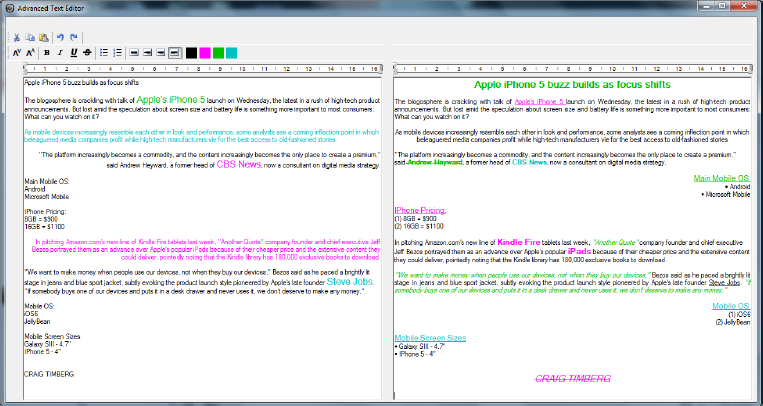
\includegraphics[width=1\linewidth]{Editor.png}
	L'interface expérimentale avec un éditeur de texte sur le côté gauche composé d'une zone de texte et d'une barre d'outils de commandes. Le format final souhaité est affiché dans la partie droite de l'éditeur de texte.
\end{center}

Les prédécesseurs ont aussi implémenté ExposeHK. Les lettres associées aux raccourcis seront affichées lorsqu'un modificateur est appuyé (Ctrl dans ce cas).
\begin{center}
	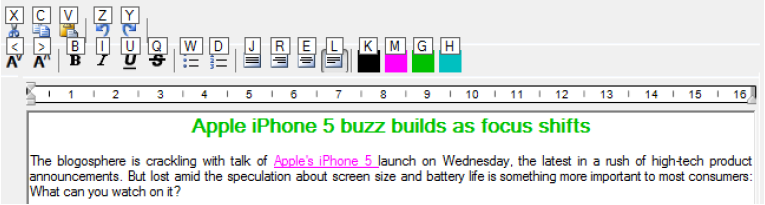
\includegraphics[width=1\linewidth]{HK.png}
	Barre d'outils avec ExposeHK activé
\end{center}
\newpage
\begin{thebibliography}{10}
	\bibitem{1} A. Cockburn, C. Gutwin, J. Scarr, et S. Malacria, «Supporting Novice to Expert
	Transitions in User Interfaces», \textit{ACM Comput. Surv.}, vol. 47, n\textdegree\ 2, p. 31:1–31:36, nov. 2014.
	\bibitem{2} J. Harrison, «Improving Users' Command Selection Performance», p.30-35, nov. 2012.
	\bibitem{3} S. Malacria, G. Bailly, J. Harrison, A. Cockburn, et C. Gutwin, «Promoting Hotkey Use
	Through Rehearsal with ExposeHK», in \textit{Proceedings of the SIGCHI Conference on Human Factors in Computing Systems}, New York, NY, USA, 2013, p. 573–582.
\end{thebibliography}
\end{document}